\documentclass{article}

% Matemática y símbolos
\usepackage{amsmath}
\usepackage{amssymb}

% Márgenes y geometría de la página
\usepackage{geometry}
\geometry{a4paper, margin=1in, bottom=2cm}

% Colores y cajas
\usepackage{xcolor}
\usepackage{mdframed}

% Gráficos y diagramas
\usepackage[T1]{fontenc}
\usepackage{tikz}
\usetikzlibrary{arrows.meta, positioning}
% Para posicionamiento relativo en TikZ

% Tablas elegantes y columnas personalizadas
\usepackage{booktabs}
\usepackage{array}
\usepackage{float}

% Imágenes
\usepackage{graphicx}

% Estilo de párrafo
\usepackage{parskip}

% Idioma
\usepackage[spanish]{babel}
\usepackage[utf8]{inputenc}  % Si no usas UTF-8 nativo

% Captions
\usepackage{caption}

% Información del documento
\title{Guía de Problemas: Cadenas de Markov y procesos estocásticos}
\author{Ricardo Largaespada}
\date{23 de abril 2025}

% Entorno personalizado para problemas
\newmdenv[
  backgroundcolor=blue!5,
  linecolor=blue,
  linewidth=1pt,
  roundcorner=5pt,
  skipabove=\baselineskip,
  skipbelow=\baselineskip
]{problem}

\begin{document}

\maketitle

%===========================================================================
%\begin{problem}
%\textbf{Problema 1: Selección de Proveedores}

%Una empresa debe elegir cada trimestre uno de tres proveedores para adquirir materia prima: \(P_1\), \(P_2\) y \(P_3\). Las probabilidades de transición dependen del proveedor seleccionado en el trimestre actual:
%\begin{itemize}
%  \item Si se trabaja con \(P_1\): 60\% de continuar con \(P_1\), 30\% cambiar a \(P_2\) y 10\% a \(P_3\).
%  \item Si se trabaja con \(P_2\): 50\% de mantener \(P_2\), 25\% cambiar a \(P_1\) y 25\% a \(P_3\).
%  \item Si se trabaja con \(P_3\): 40\% de mantener \(P_3\), 40\% cambiar a \(P_1\) y 20\% a \(P_2\).
%\end{itemize}

%\textbf{Tareas:}
%\begin{enumerate}
%    \item Construir la matriz de transición \(T\).
%    \item Determinar la probabilidad de que en 2 trimestres se pase de \(P_1\) a \(P_3\) (calcular \( (T^2)(1,3) \)).
%    \item Analizar si existen estados transitorios o si todos son recurrentes.
%\end{enumerate}
%\end{problem}
%===========================================================================

\begin{problem}
\textbf{Problema 1: Evolución de la Satisfacción del Cliente}

Una compañía de telecomunicaciones clasifica a sus clientes en tres categorías de satisfacción:
\(\mathbf{S}\): Satisfecho, \(\mathbf{N}\): Neutral e \(\mathbf{I}\): Insatisfecho.

La evolución de la satisfacción del cliente se modela mediante una cadena de Markov, en la cual la probabilidad de transición de un estado a otro en cada período se representa mediante la siguiente matriz de transición \(P\):

\[
P = \begin{pmatrix}
0.70 & 0.20 & 0.10 \\
0.30 & 0.40 & 0.30 \\
0.20 & 0.30 & 0.50 \\
\end{pmatrix}.
\]

La distribución inicial (o vector de probabilidad) de la satisfacción de los clientes es: \(\mathbf{p}^{(0)} = \begin{pmatrix} 0.60 \\ 0.30 \\ 0.10 \end{pmatrix}.\)

\textbf{Tareas:}
\begin{enumerate}
    \item ¿Cuál es la proporción estimada de clientes que se espera estén en cada una de las categorías (Satisfecho, Neutral, Insatisfecho) después de 4 períodos?
\end{enumerate}
\end{problem}
%===========================================================================

\begin{problem}
\textbf{Problema 2: Estimación de la Matriz de Transición a partir de una Sucesión de Clics}

En un portal web se ha registrado la secuencia de páginas visitadas por un usuario durante una sesión. Las tres secciones del portal se identifican como:
\[
\textbf{I}: \text{Inicio}, \quad \textbf{N}: \text{Noticias}, \quad \textbf{F}: \text{Foro}.
\]
La siguiente es la secuencia observada (en orden cronológico) de clics:
\[
I,\; N,\; I,\; F,\; I,\; I,\; N,\; F,\; F,\; I,\; N,\; F,\; I,\; I,\; N,\; I,\; F,\; N,\; I,\; F.
\]
\textbf{Tareas:}
\begin{enumerate}
    \item \textbf{Construir la matriz de transición empírica:}  
    \begin{enumerate}
        \item A partir de la secuencia dada, cuente cuántas veces se produce cada transición (por ejemplo, de \(I\) a \(N\), de \(N\) a \(F\), etc.).
        \item Utilice estos conteos para estimar las probabilidades de transición, es decir, divida el número de transiciones desde un estado \(X\) a un estado \(Y\) entre el total de transiciones salientes del estado \(X\). Arme la matriz \(T\) de dimensión \(3 \times 3\) en el orden \(\{I, N, F\}\).
    \end{enumerate}

    \item \textbf{Verificar la propiedad de estocasticidad:}  
    Compruebe que la suma de las probabilidades en cada fila de la matriz \(T\) es 1.
    
    \item \textbf{Interpretar la matriz:}  
    Explique brevemente qué indica cada elemento \(t_{XY}\) de la matriz en el contexto del comportamiento de navegación del usuario.

%    \item \textbf{Utilizando las ecuaciones de Chapman--Kolmogorov:}  
%    Calcule la matriz de transición en 2 pasos, \(T^2\), y explique qué información proporciona respecto a la navegación del usuario.
    
\end{enumerate}

\end{problem}
%============================================================================

%\begin{problem}
%\textbf{Problema 4: Visita a Páginas Web (Estados Periódicos)}

%Un usuario navega en un portal web con tres secciones: \textbf{Inicio (I)}, \textbf{Noticias (N)} y \textbf{Foro (F)}. Las probabilidades de transición en cada clic son:
%\begin{itemize}
%    \item Desde \textbf{I}: 0.5 de ir a \textbf{N} y 0.5 a \textbf{F}.
%    \item Desde \textbf{N}: 0.3 de regresar a \textbf{I}, 0.2 de ir a \textbf{F} y 0.5 de quedarse en \textbf{N}.
%    \item Desde \textbf{F}: 0.8 de regresar a \textbf{I} y 0.2 de quedarse en \textbf{F}.
%\end{itemize}

%\textbf{Tareas:}
%\begin{enumerate}
%    \item Construir la matriz de transición.
%    \item Calcular las matrices \(T^2\) y \(T^3\).
%    \item Analizar cada estado (\textbf{I}, \textbf{N}, \textbf{F}): ¿es recurrente o transitorio? ¿Es periódico o aperiódico?
%    \item Si el usuario inicia en \textbf{Inicio (I)}, determinar la probabilidad de que visite \textbf{Foro (F)} al menos una vez en los próximos 4 clics.
%\end{enumerate}
%\end{problem}
%===========================================================================

\begin{problem}
\textbf{Problema 3: Cadena con Estado Absorbente (Fallas de un Sistema)}

Un sistema de cómputo puede encontrarse en uno de los siguientes estados:
\begin{enumerate}
    \item \textbf{Funcionando Normal (N)}
    \item \textbf{Funcionando con Falla Parcial (F)}
    \item \textbf{En Mantenimiento (M)}
    \item \textbf{Irreparable (I)} (estado absorbente, ya que una vez en este estado no se sale)
\end{enumerate}

La matriz de transición de un paso se propone como:
\[
T = \begin{pmatrix}
0.6 & 0.3 & 0.1 & 0 \\
0.2 & 0.4 & 0.3 & 0.1 \\
0.1 & 0.3 & 0.5 & 0.1 \\
0   & 0   & 0   & 1
\end{pmatrix}
\]

\textbf{Tareas:}
\begin{enumerate}
%    \item Verificar que \(T\) es estocástica (cada fila debe sumar 1).
    \item Calcular la probabilidad de que el sistema se encuentre en \textbf{Irreparable (I)} dentro de 2 pasos, partiendo de \textbf{Normal (N)}.
    \item Determinar si el estado \textbf{Irreparable (I)} es efectivamente un estado absorbente.
    \item Calcular \(T^n\) (al menos de forma teórica o con un software) y describir el límite cuando \( n \to \infty \).
    \item Concluir: ¿El sistema necesariamente llegará a ser irreparable con probabilidad 1?
\end{enumerate}
\end{problem}
%===========================================================================

%\begin{problem}
%\textbf{Problema 4: Juego de Azar}

%Un jugador inicia con 2 fichas y puede llegar a un máximo de 4 o perderlo todo (0 fichas). Al final de cada jugada:
%\begin{itemize}
%    \item Gana 1 ficha con probabilidad 0.4.
%    \item Pierde 1 ficha con probabilidad 0.6.
%\end{itemize}
%Una vez que alcanza 4 fichas, se retira (estado absorbente) y, si llega a 0, pierde (otro estado absorbente). Se consideran los estados: \(0,1,2,3,4\). Cada uno representa la cantidad de fichas que el jugador tiene.

%\textbf{Tareas:}
%\begin{enumerate}
%    \item Construir la matriz de transición.
%    \item Partiendo de 2 fichas, calcular la probabilidad de que eventualmente el jugador llegue a 4 fichas (gane) en lugar de 0 (pierda).
%    \item Definir si los estados \(1\), \(2\) y \(3\) son transitorios o recurrentes.
%    \item Discutir la existencia (o no) de una distribución estacionaria teórica en presencia de dos estados absorbentes; ¿qué se concluye sobre la dinámica a largo plazo?
%\end{enumerate}
%\end{problem}
%===========================================================================

\begin{problem}
\textbf{Problema 4: Análisis de Periodicidad y Recurrencia}

Considera la siguiente matriz de transición de una cadena con 5 estados \(\{1,2,3,4,5\}\):
\[
T = \begin{pmatrix}
0   & 1   & 0   & 0   & 0 \\
1   & 0   & 0   & 0   & 0 \\
0.6 & 0   & 0.2 & 0.2 & 0 \\
0   & 0   & 0   & 1   & 0 \\
0   & 0   & 0   & 0.8 & 0.2 
\end{pmatrix}
\]

\textbf{Tareas:}
\begin{enumerate}
    \item Identificar si existe algún estado absorbente.
    \item Determinar la periodicidad de cada estado (calcular el máximo común divisor (gcd) de los enteros \(n\) tales que \((T^n)(i,i) > 0\)).
    \item Clasificar los estados en recurrentes y transitorios (analizando las probabilidades de retorno).
    \item Realizar una simulación en MATLAB para corroborar las conclusiones sobre la dinámica.
\end{enumerate}
\end{problem}
%===========================================================================

\begin{problem}
\textbf{Problema 5: Producción en una Fábrica}

Se consideran cuatro estados en una línea de producción: \textbf{Diseño (D)}, \textbf{En Producción (P)}, \textbf{Control de Calidad (C)} y \textbf{Producto Terminado (T)}.

\begin{center}
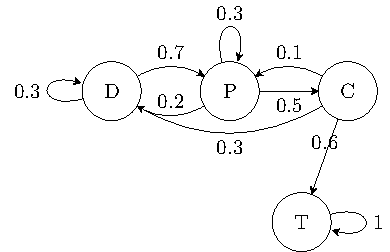
\includegraphics[scale=1]{images/trabajo03-1.pdf}
\end{center}

\textbf{Tareas:}
\begin{enumerate}
    \item Escribir la matriz de transición \(T\).
    \item Si la producción inicia en \textbf{D}, determinar la probabilidad de llegar a \textbf{T} en exactamente 3 pasos.
    \item Calcular la probabilidad de que el producto sea terminado (\textbf{T}) en algún momento; discutir si la terminación ocurre con probabilidad 1.
    \item Identificar si existen estados transitorios, aparte del estado absorbente \textbf{T}, y explicar.
    \item Comentar: Si se realizan múltiples simulaciones, ¿se espera que todos los productos eventualmente se terminen?
\end{enumerate}
\end{problem}

%============================================================================
\begin{problem}
\textbf{Problema 6: Análisis de Préstamos con Retraso en Pagos }

Un banco ofrece préstamos a 1 año de plazo (4 trimestres). Cada trimestre, el cliente puede:
\begin{itemize}
    \item Pagar a tiempo, manteniéndose o regresando al estado de “0 trimestres de retraso”.
    \item Incurrir o persistir en mora, avanzando a “1 trimestre de retraso”, “2 trimestres de retraso”, etc.
    \item Si el préstamo alcanza “4 trimestres de retraso”, el banco lo considera incobrable y lo cancela (estado absorbente).
\end{itemize}

Su departamento de créditos ha recopilado la siguiente información para caracterizar la evolución de un préstamo a lo largo de cada trimestre:
\begin{enumerate}
    \item Si el crédito está al corriente (0 trimestres de retraso) al inicio de un trimestre, existe un 85\% de probabilidad de que continúe al corriente, un 10\% de que salte a “1 trimestre de retraso” y un 5\% de que vaya directamente a “2 trimestres de retraso” (caso de un pago muy retrasado).
    \item Si el crédito se encuentra en “1 trimestre de retraso”, existe un 50\% de probabilidad de que se ponga al corriente al siguiente trimestre (0 trimestres de retraso), 30\% de que permanezca en “1 trimestre de retraso” y 20\% de que avance a “2 trimestres de retraso”.
    \item Estando en “2 trimestres de retraso”, hay 25\% de probabilidad de que el cliente regularice su situación (regresando a 0 trimestres de retraso), 25\% de permanecer en “2 trimestres de retraso” y 50\% de pasar a “3 trimestres de retraso”.
    \item Si el préstamo está ya en “3 trimestres de retraso”, entonces con probabilidad 10\% se logra regularizar (0 trimestres de retraso), con 40\% permanece en “3 trimestres de retraso” y con 50\% avanza a “4 trimestres de retraso”.
    \item Alcanzar “4 trimestres de retraso” implica que el préstamo es declarado incobrable y cancelado: se trata de un estado absorbente (\(100\%\) de probabilidad de quedarse en 4 trimestres de retraso).
\end{enumerate}

\textbf{Tareas:}
\begin{enumerate}
    \item \textbf{Construir la matriz de transición.} Denote los estados como:
    \[
    E_0:\; 0 \text{ trimestres de retraso}, \quad 
    E_1:\; 1 \text{ trimestre de retraso}, \quad
    E_2:\; 2 \text{ trimestres de retraso}, \] 
    \[E_3:\; 3 \text{ trimestres de retraso}, \quad
    E_4:\; 4 \text{ trimestres de retraso (incobrable)}.
    \]
    \item \textbf{Verificar si la matriz es estocástica.} (Es decir, que la suma de cada renglón sea 1).
    \item \textbf{Analizar si alguno de los estados es absorbente y justificar.}  
    \item \textbf{Calcular la probabilidad de que un préstamo que inicia en 2 trimestres de retraso llegue a ser incobrable en 2 pasos.} (Esto corresponde a evaluar \((T^2)(2,4)\).)
    \item \textbf{Discuta si los estados \(E_1, E_2\) y \(E_3\) son transitorios o recurrentes.} Mencione los criterios teóricos para clasificarlos.
\end{enumerate}
\end{problem}
%============================================================================

%============================================================================
\begin{problem}
\textbf{Problema 7: Mantenimiento de Equipos de Producción}

En una planta industrial se tiene un equipo cuya condición se clasifica en tres estados:
\[
O:\; \text{Operativo}, \quad M:\; \text{En Mantenimiento}, \quad F:\; \text{Con Falla (Incobrable)}.
\]
El comportamiento del equipo se modela mediante una cadena de Markov. En cada período (por ejemplo, un mes) se presentan las siguientes probabilidades de transición:

\begin{itemize}
    \item Desde el estado \textbf{Operativo} (\(O\)):
    \begin{itemize}
        \item Se mantiene operativo con probabilidad 0.80.
        \item Pasa a estar en mantenimiento con probabilidad 0.15.
        \item Se detecta una falla que lo deja inoperativo con probabilidad 0.05.
    \end{itemize}
    \item Desde el estado \textbf{En Mantenimiento} (\(M\)):
    \begin{itemize}
        \item El equipo es reparado y vuelve a estar operativo con probabilidad 0.70.
        \item Permanece en mantenimiento con probabilidad 0.20.
        \item La falla se agrava, derivando en un estado de falla permanente con probabilidad 0.10.
    \end{itemize}
    \item Desde el estado \textbf{Con Falla} (\(F\)):
    \begin{itemize}
        \item Se asume que la falla es definitiva; por lo tanto, el equipo permanece en \(F\) con probabilidad 1.
    \end{itemize}
\end{itemize}

\textbf{Tareas:}
\begin{enumerate}
    \item \textbf{Construir la matriz de transición} \(T\). Use el siguiente orden de estados:
    \[
    E_1 = O,\quad E_2 = M,\quad E_3 = F.
    \]
    Escriba la matriz \(T\) en forma de una matriz \(3 \times 3\) cuyos elementos \(t_{ij}\) representan la probabilidad de pasar del estado \(E_i\) al estado \(E_j\).
    
    \item \textbf{Verificar que la matriz es estocástica.} Es decir, compruebe que la suma de las probabilidades de cada fila es igual a 1.
    
    \item \textbf{Utilizando las ecuaciones de Chapman–Kolmogorov, calcular la matriz de transición en 2 pasos} \(T^2\).
    
    \item \textbf{Determinar la probabilidad de que el equipo, partiendo en estado \(O\), esté en estado \(F\) después de 2 períodos.} Esto corresponde a evaluar \((T^2)(1,3)\).
    
    \item \textbf{Analizar los estados:}  
    \begin{enumerate}
        \item Identifique si el estado \(F\) es absorbente y justifique su respuesta.
        \item Discuta, basándose en la estructura de la matriz, si los estados \(O\) y \(M\) son recurrentes o transitorios y si presentan comportamiento periódico o aperiódico.
    \end{enumerate}
\end{enumerate}
\end{problem}
%============================================================================

\end{document}
